\section{Linear Inequalities}

\subsection{Review problems}

\begin{enumerate}
\item Solve each of the following inequalities, expressing the solution set in interval notation and graphing the solution set on a number line.
\begin{enumerate}
\item $x > -1$
\item $2x + 5\leq 7$
\item $7 - 3x < 5x - 9$
\item $(x + 4)^2 + x^2\geq (x + 2)^2 + (x + 1)^2$
\end{enumerate}
\item For each of the following combinations of inequalities, write the solution set in interval notation and graph the solution set on a number line.
\begin{enumerate}
\item $2\leq 3 + x < 6$
\item $x\geq 2 - x$ or $5 - 3x\geq x + 9$
\item $-9x + 4 < 8x + 2 < 2x + 7$
\item $-6x - 8\leq 4$ and $-x - 10\leq -7$
\item $-6x - 8\leq 4$ or $-x - 10\leq -7$
\end{enumerate}
\item \begin{enumerate}
\item Write down a pair of linear inequalities, each involving a single variable $x$, for which no real number satisfies both of the inequalities simultaneously. In this case, the solution set for ``[first inequality] and [second inequality]'' is the \emph{empty set}, denoted $\emptyset$.
\item Write down a pair of linear inequalities, each involving a single variable $x$, for which every real number satisfies at least one of the inequalities. In this case, the solution set for ``[first inequality] or [second inequality]'' is the entire set of real numbers, denoted $\mathbb{R}$. We could also write $(-\infty, \infty)$.
\item Write down a pair of linear inequalities, each involving a single variable $x$, for which the only real number which does not satisfy at least one of the inequalities is $6.626$. Express this solution set in interval notation as a union ($\cup$) of two intervals.
\end{enumerate}
\item Solve each of the following inequalities, expressing the solution set in interval notation and graphing the solution set on a number line.
\begin{enumerate}
\item $\lvert x\rvert < 4$
\item $\lvert x - 4\rvert\geq 2$
\end{enumerate}
\item Graph the solution set of each of the following inequalities.
\begin{enumerate}
\item $x + y < -2$
\item $3x - y\geq 7$
\item $(x - 1)^2 + y^2\leq (x - 5)^2 + (y - 2)^2$
\item $\lvert x\rvert + \lvert y\rvert < 1$
\end{enumerate}
\item Graph the solution set of each of the following combinations of inequalities.
\begin{enumerate}
\item $x + y\leq -2$ and $3x - y > 7$
\item $x + y < -2$ or $3x - y > 7$
\item $2x + 3y\geq 4$ and $6y\leq 12 - 4x$
\item $3x + 3y < -5x < 5y$
\end{enumerate}
\item Supposing $a\leq b$ and $c\leq d$, which of the following must also be true?
\begin{enumerate}
\item $a + c\leq b + d$
\item $a - c\leq b - d$
\item $ac\leq bd$
\item $a/c\leq b/d$
\end{enumerate}
For the statements that were not guaranteed to be true, which ones are guaranteed to be true when we also assume $a\geq 0$ and $c\geq 0$?
\end{enumerate}


\subsection{Challenge problems}

\begin{enumerate}[resume]
\item Write down three inequalities for which the set of all points $(x,y)$ satisfying all of the three inequalities is the set shown below.
\begin{center}
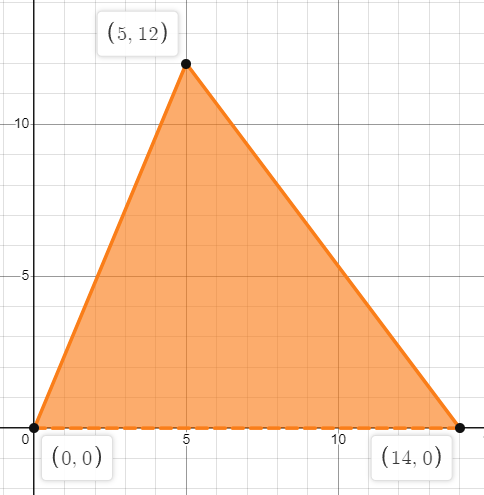
\includegraphics[scale=0.4]{lin-ineq-triangle.png}
\end{center}
\item Miko and Yuu plan to sell alms bowls and cowrie shell necklaces at their school's culture festival. Each bowl sold earns them \$30 while each necklace sold earns them \$23. Their stand will allow them to stock up to 120 items in total, and the amounts of these two items cannot differ by more than 40. (Otherwise, Miko and Yuu will start arguing so much that they drive away all potential customers.) To make the items, they need to borrow materials from the art club. Each bowl uses up 2\% of the material allowance that the art club gives them, while each necklace uses up 1\% of that allowance. Given all of these restrictions, what is the maximum possible amount of revenue that Miko and Yuu could bring in?
\item Find all values of $x$ for which
\begin{equation*}
\lvert\lvert x - 1\rvert - \lvert 2x - 8\rvert\rvert\leq 6.
\end{equation*}
Express your answer in interval notation.
\end{enumerate}


\newpage
\subsection{Answers}

In all instances of interval notation, writing $\infty$ in place of $+\infty$ would be valid (but writing $\infty$ in place of $-\infty$ would not).

\begin{enumerate}
\item \begin{enumerate}
\item $(-1, +\infty)$
\begin{center}
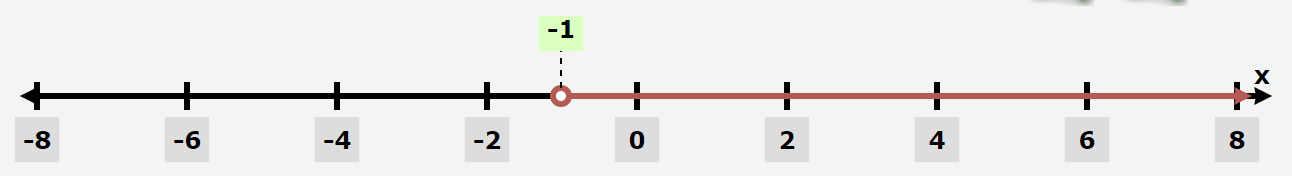
\includegraphics[scale=0.5]{lin-ineq-ans-1a.png}
\end{center}
\item $(-\infty, 1]$
\begin{center}
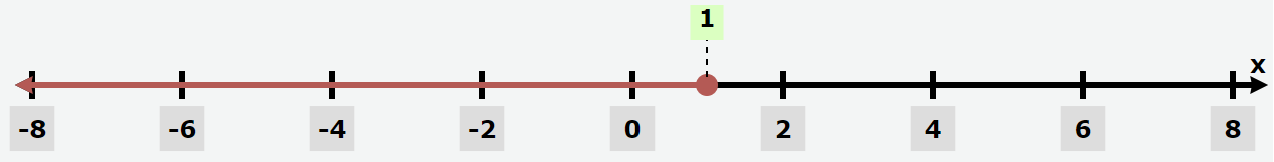
\includegraphics[scale=0.5]{lin-ineq-ans-1b.png}
\end{center}
\item $(2, +\infty)$
\begin{center}
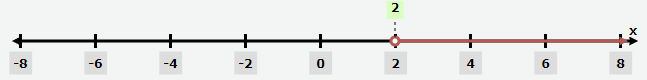
\includegraphics[scale=0.5]{lin-ineq-ans-1c.png}
\end{center}
\item $[-11/2, +\infty)$
\begin{center}
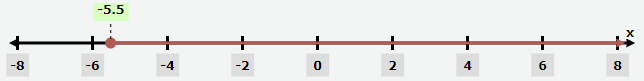
\includegraphics[scale=0.5]{lin-ineq-ans-1d.png}
\end{center}
\end{enumerate}
\item \begin{enumerate}
\item $[-1,3)$
\begin{center}
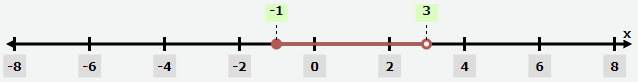
\includegraphics[scale=0.5]{lin-ineq-ans-2a.png}
\end{center}
\item $(-\infty,-1]\cup [1,+\infty)$
\begin{center}
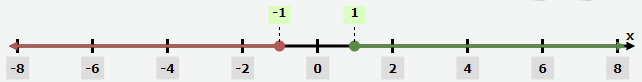
\includegraphics[scale=0.5]{lin-ineq-ans-2b.png}
\end{center}
(The colors on the graph are irrelevant.)
\end{enumerate}
\item 
\end{enumerate}